%------------------------------------------------
\section{Фазовые колебания}

\begin{frame}
	\frametitle{Фазовые колебания в резонансных ускорителях. Принцип автофазировки}
	\par Принцип фазовой фокусировки синхротронного движения был открыт Макмилланом и Векслером в 1944-1945 гг. 
	\newline
	\par Открытие фазовой стабильности проложило путь для всех современных ускорителей высоких энергий, называемых “синхротронами”, и после полувека исследований и разработок оно остается краеугольным камнем современных ускорителей. Кроме того, пучти могут быть укорочены, удлинены, объединены или сгруппироваными для достижения многих целей с помощью ВЧ манипуляции.
\end{frame}

%------------------------------------------------
\begin{frame}
	\frametitle{Уравнения движения}
	
	\par Поле от ВЧ станции
	\begin{equation}
		\mathcal{E}=\mathcal{E}_0 \sin \left(\phi_{\mathrm{rf}}(t)+\phi_{\mathrm{s}}\right), \quad \phi_{\mathrm{rf}}=h \omega_0 t
	\end{equation}
	
	\par Уравнение движения для разности энергий становится
	\begin{equation}
		\frac{d}{d t}\left(\frac{\Delta E}{\omega_0}\right)=\frac{1}{2 \pi} e V\left(\sin \phi-\sin \phi_{\mathrm{s}}\right)
	\end{equation}
	
	\par Для фазы
	\begin{equation}
		\dot{\phi}=h \omega_0 \eta \delta=\frac{h \omega_0^2 \eta}{\beta^2 E}\left(\frac{\Delta E}{\omega_0}\right)
	\end{equation}
	

\end{frame}

%------------------------------------------------
\begin{frame}
	\frametitle{}
  	\par Линеаризованное уравнение движения
  	
  	\begin{equation}
  		\frac{d^2}{d t^2}\left(\phi-\phi_s\right)=\frac{h \omega_0^2 e V \eta_0 \cos \phi_s}{2 \pi \beta^2 E}\left(\phi-\phi_s\right)
  	\end{equation}
  	
  	\par Условие стабильности
  	
  	\begin{equation}
  		\eta_0 \cos \phi_s < 0
  	\end{equation}
  	
  	\begin{figure}
  		\centering
  		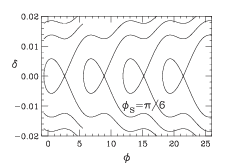
\includegraphics[width=0.3\linewidth]{images/synchr}
  	\end{figure}
  	
	 
\end{frame}